\section{Smooth 0--1 Loss Approximation Approach}
\label{cha:Smoothlossapprox}

Most of algorithms in previous chapters aim at determining the exact solution of the 0--1 loss optimization problem. The guarantee of the returned solution being optimal comes at a cost, that is the running time of these algorithms is significant. To reduce the running time, the combinatorial search approximation (CSA) algorithm was proposed in Chapter \ref{cha:combinatorialsearch}, which has complexity $O(N^3D^2)$ and is sensitive to dimensionality. In this chapter, a more efficient approximation algorithm is being studied. This time, the approximation is based on a smooth approximation to the 0--1 loss function, with controllable smoothness and precision. This approximation is detailed in Section \ref{sec:sla.foundation}, where necessary mathematical foundation to develop the smooth loss approximation (SLA) algorithm is also developed. Section \ref{sec:sla.algorithm} then presents the SLA algorithm in detail, with a complexity analysis provided in the section after that. Finally, the last section of this chapter summarizes advantages, disadvantages, and concludes the smooth loss approximation approach.

%=================================================
\subsection{Foundation of Smooth 0--1 Loss Approximation}
\label{sec:sla.foundation}

This section develops the necessary foundation for the smooth loss approximation approach. To give an overview, the main idea behind the smooth loss approximation is summarized as follows. A differentiable function with controllable approximation's precision and smoothness is developed to approximate the 0--1 loss function. This approximating function shall be referred to as the \emph{smooth loss function}. The optimal 0--1 loss solution is then approximated by the solution of the smooth loss function, which is obtained by optimizing that function at increasing level of approximation's precision. The remaining paragraphs of this section concentrates on developing the smooth loss function and providing a sketch of the SLA algorithm. 

\begin{figure}[here]
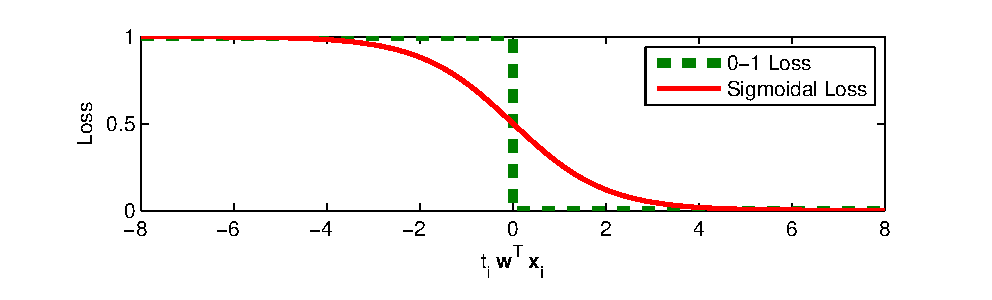
\includegraphics[width=0.50\textwidth]{images/fig51_sigmoid.eps}
\caption{
This plot illustrates how sigmoidal loss approximates 0--1 loss. As can be seen, sigmoidal loss is quite similar to 0--1 loss except that it makes a continuous transition from 1 to 0 around 0.
}
\label{fig:sla.sigmoid}
\end{figure}

The definition of 0--1 loss optimization problem given in Section \ref{sec:bgr.formulation} of Chapter \ref{cha:background} stated the 0--1 loss function as 
$$L(\w) = \sum_{i=1}^N l_i = \sum_{i=1}^N \mathbb{I} [t_i \w^T \xi \leq 0],$$
and the optimal solution is a weight vector $\w^*$ that minimizes the 0--1 loss function above. It has been also discussed, that  0--1 loss is non-differentiable non-smooth non-convex function with complicated shape, as illustrated by Figure \ref{fig:complex_shape}. To develop the smooth loss function that approximates the 0--1 loss function above, the individual loss $l_i = \mathbb{I} [t_i \w^T \xi \leq 0]$ of data point $\xi$ is now being examined. It is known that this individual 0--1 loss can be approximated by sigmoidal loss as follows:
$$l_i = \mathbb{I} [t_i \w^T \xi \leq 0] \approx \frac{1}{1 + e^{t_i \w^T \xi }}.$$
This approximation is illustrated by Figure \ref{fig:sla.sigmoid}, where it can be seen, that sigmoidal loss is quite similar to 0--1 loss except that it makes a continuous transition from 1 to 0 around $t_i \w^T \xi = 0$. 

As the smooth loss function being developed here requires controllable smoothness and approximation's precision, a positive constant $K \in \R^+$ is multiplied into the exponential term of the sigmoidal loss. Then, the approximation becomes
$$l_i = \mathbb{I} [t_i \w^T \xi \leq 0] \approx \frac{1}{1 + e^{Kt_i \w^T \xi }}.$$
For convenience, this new approximation shall be referred to as \emph{smooth loss}, and the constant $K$ referred to as the \emph{precision constant}. The advantage of smooth loss is that the precision and smoothness of the approximation can be controlled, because as $K$ gets bigger, the approximation approaches the true 0--1 loss, while the smoothness is reduced. In fact, the following asymptotic formula can be proven easily (assuming $\xi$ does not lie directly on the decision hyperplane):
$$\lim_{K \rightarrow +\infty} \frac{1}{1 + e^{Kt_i \w^T \xi }} = l_i.$$

\begin{figure}[here]
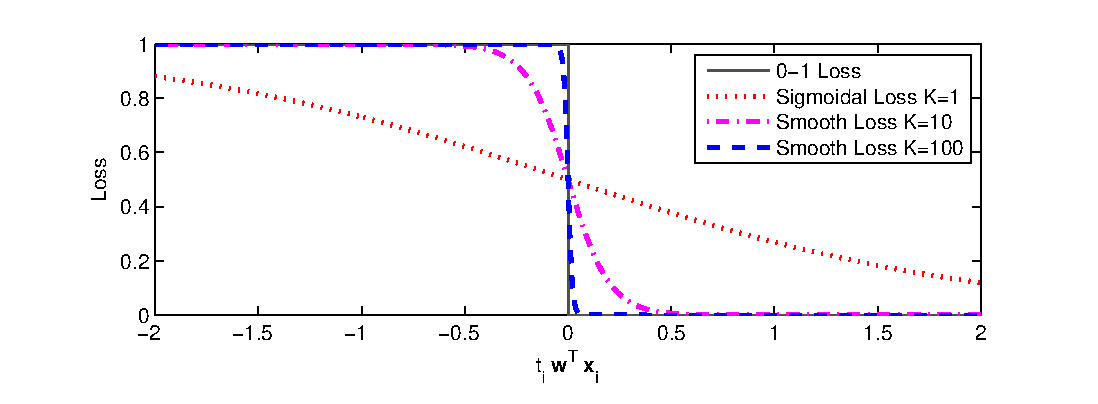
\includegraphics[width=0.50\textwidth]{images/fig52_smooth.eps}
\caption{
This plot illustrates how smooth loss approximates 0--1 loss. As can be seen, for precision constant $K=100$, smooth loss almost approximates 0--1 loss exactly, with abrupt changes around 0, whereas for $K=1$, smooth loss is exactly sigmoidal loss, and it is much smoother comparing to $K=100$. For $K=10$, the smoothness and precision fit in between the two previous cases. 
}
\label{fig:sla.smooth}
\end{figure}

This discussion is supported by Figure \ref{fig:sla.smooth}, where the smooth loss is drawn at different values of the precision constant $K=1, 10, 100$ corresponding to the red, magenta, and blue curve. The gray curve displays the 0--1 loss for comparison. It can be seen, that for $K=100$, the smooth loss is already very close to the 0--1 loss, and it also displays less smoothness (i.e., abrupt changes around 0), whereas for $K=1$, the smooth loss is exactly the sigmoidal loss, with a smooth transition around 0.


\begin{figure}[here]
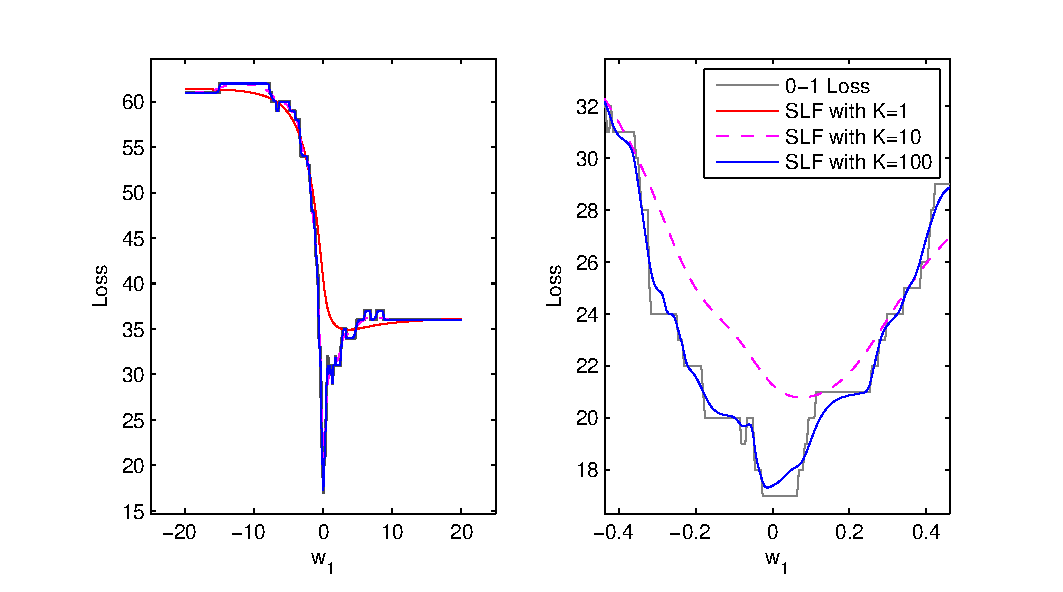
\includegraphics[width=0.50\textwidth]{images/fig53_smoothfunction.eps}
\caption{
This figure illustrates how smoothness and precision of the smooth loss function (SLF) changes with different values of constant $K$. The plot on the right is a close-up of the plot on the left around global minimum. The value of the smooth loss function is plotted versus changes of one component, $w_1$, of the weight vector $\w$ around the minimum (all other components are fixed). The blue curve corresponds to $K=100$, the red curve corresponds to $K=1$, the magenta curve corresponding to $K=10$, the gray curve is the true 0--1 loss displayed for comparison. For $K=1$, the function is smooth with only two extrema as shown by the red curve on the left plot. For $K=100$, there are many local optima and the smooth loss function closely approximates 0--1 loss function as shown by the blue curve in both plots. For $K=10$, many local optima are smoothed out, but many extrema still present, as shown by the magenta curve visible on the right plot (not apparent in the left plot due to the scale).
}
\label{fig:sla.smoothfunction}
\end{figure}

It is now possible to define the \emph{smooth loss function} as the sum of the smooth losses of all data point as follows:
$$L_K(w) = \sum_{i=1}^N \frac{1}{1 + e^{Kt_i \w^T \xi }}.$$
Figure \ref{fig:sla.smoothfunction} illustrates how this smooth loss function changes with different values of the precision constant $K$. The dataset underlying this figure has 100 points in $\R^3$. The curves in the figure represent the smooth loss function as a function of  component $w_1$ of the loss vector (other components are held fixed). The figure is divided into two plots. The plot on the left shows the general shapes of smooth loss function at different values of $K=1, 10, 100$ corresponding to the red, magenta, blue curves. The plot on the right is the close-up of the plot on the left and shows the detailed shape of smooth loss functions around the minimum. It also shows the true 0--1 loss (gray curve) for reference. As can be seen, for $K=1$, the smooth loss function (the red curve in the left plot) is very smooth with only two extrema, while on the other hand, for $K=100$ the function follows quite closely to the the 0--1 loss function, which means it has lots of local optima corresponding to abrupt changes of the 0--1 loss function, for $K=10$ (corresponding to the magenta curve on the right plot, not very apparent on the left plot), the local optima is smoothed out, but many extrema still present. There are two important things to note here. Firstly, the minimum of the smooth loss function evaluated at different value of $K$ are relatively close to each other, and as $K$ increases, it approaches the 0--1 loss minimum. Secondly, although at high precision there is a lot of local optima in the shape of the smooth loss function, but the general trend is a valley-like or canyon-like shape. These notes give rise to the idea behind the smooth loss approximation approach, which has the following sketch:  

\begin{description}
\setlength{\itemsep}{0cm}
\setlength{\parskip}{0cm}
\item[Step 1:] \hfill \\ Find the optimal solution, $\w^*$, of the smooth loss function corresponding to a small value of $K$ (e.g., $K=1$) in a wider range (radius) around some initially approximated value of $\w$. 
\item[Step 2:] \hfill \\ Use the previously found optimal solution as the initial approximation to start the search for the new minimum of the smooth loss function corresponding to an increased precision constant $K$ (e.g., K=10, 100, \dots) and reduced search radius (e.g., by a half). This step is repeated again and again until a desired level of the precision has been reached (e.g., $K=1000$). 
\item[Step 3:] \hfill \\ The last optimal solution, $\w^*$, found in Step 2, which is the one corresponding to the desired level of precision, is returned as the approximation to the optimal solution of 0--1 loss. 
\end{description}

This is, of course, just a very rough idea and many things need to be clarified. The most important thing is perhaps the range optimization process: given a precision constant $K$, a radius $R$, an initial guess $\w$, how to efficiently find the optimal solution, $\w^*$, of the corresponding smooth loss function? The algorithm for this is being detailed in the first subsection of the next section. Other things to be clarified are, for examples, how to determine the initial approximation in Step 1? What is the suitable way to increase the precision constant and reduce the search radius? These are being address in the second subsection of the next section, where the SLA algorithm is detailed. 

%=================================================
\subsection{Smooth Loss Approximation Algorithm}
\label{sec:sla.algorithm}

The previous section provided a sketch of the SLA algorithm and left some  some open problems to be answered. Among those, the range optimization process was identified as having a crucial importance to the  development of the SLA algorithm. This section, therefore, concretize the SLA algorithm firstly by providing a specialized algorithm for the range optimization process in the first subsection. The subsection after that, then, provides and discusses the detailed SLA algorithm.  

%===========================
\subsubsection{Range Optimization}
\label{ssec:sla.range}

All steps in the sketch of the smooth loss approximation algorithm given in the previous section repeatedly rely on a range optimization process, which is described as follows. Given a radius $R$, a precision constant $K$, and an initial value of $\w$, find the minimum of the smooth loss function evaluated with the given value of $K$ in the given radius $R$ around the given initial approximation $\w$. This subsection, therefore, aims at providing an algorithm tailored for this task. 

Note, that the smooth loss function is differentiable, but not convex. Moreover, there may be many local minima when the smoothness is low (i.e., when precision constant is high). Thus, finding the exact minimum in the given range is hard. So, an approximation will be given instead. There are a number of methods that can be used in this situation, such as simulated annealing \cite{Kirkpatrick}, or even genetic algorithm \cite{Goldberg}. These, however, are generic methods, which take a long time to find good approximation, and do not exploit the structure of the smooth loss function as discussed in the previous section. Therefore, a specialized approximation algorithm is being proposed for the range optimization process. The proposing algorithm is a mixture of the gradient descent method \cite{Cauchy}, the pattern search method \cite{Hooke}, and the hill climbing heuristic. It, thus, possesses advantages of all these methods. This algorithm is detailed in Algorithm \ref{alg:sla.range}, and a step by step description is being given next. 

\begin{figure}
\caption{
Range Optimization Algorithm for Smooth Loss Function. \\
\text{\hspace{2.1cm}} $Input$: Initial guess $\w$, precision constant $K$, radius $R$, step size $\epsilon_S$. \\
\text{\hspace{2.1cm}} $Output$: Approx. optimal solution $\w^*$ corresp. to given parameters.
}
\label{alg:sla.range}
\begin{algorithmic}[1]
\Function{Gradient-Descent-in-Range}{$\w, K, R, \epsilon_S$} \Comment{returns $\w^*$}
\Repeat
   \Statex \Comment{{\bf Stage 1}: Use modified gradient descent to find a local minimum}
   \State $\w^* \gets \w$
   \Repeat
      \State $r \gets max_{rate}$
      \State $\w \gets (\w^* - r \nabla L_K(\w^*))$
      \While{$(r \geq min_{rate}) \land (L_K(\w^*) - L_K(\w) < \epsilon_L) $}
         \State $r \gets 0.1 r$
         \State $\w \gets (\w^* - r\nabla L_K(\w^*))$
      \EndWhile
      \If{$r \geq min_{rate}$}
         \State $\w^* \gets \w$
      \EndIf
   \Until{$(-\epsilon_G \preccurlyeq  \nabla L_K(\w^*) \preccurlyeq \epsilon_G) \lor (r < min_{rate})$}
   \Statex \Comment{{\bf Stage 2}: Probe within radius $R$ to escape the local minimum}
   \For {$i=0$ to $D$}
      \For{$step \in \{\epsilon_S, -\epsilon_S, 2\epsilon_S, -2\epsilon_S, \dots, R, -R \}$}
         \State $\w \gets \w^*$  
         \State $w_i \gets w_i + step$
         \If{$L_K(\w^*) - L_K(\w) \geq \epsilon_L$}
            \State {\bf break both for loops and repeat from step 3}
         \EndIf       
      \EndFor
   \EndFor
   \Statex
\Until{$L_K(\w^*) - L_K(\w) < \epsilon_L$}
\State \Return $\w^*$
\EndFunction
\end{algorithmic}
\end{figure}

The detailed description of Algorithm \ref{alg:sla.range} is as follows. In step 1, the function {\sc Gradient-Descent-in-Range} takes as input an initial approximation $\w$, a specific precision constant $K$, a radius $R$, a step size $\epsilon_S$ specifying distance of probing points in the search range given by radius $R$, and returns an approximated optimal solution $\w^*$ minimizing the smooth loss loss function with the given input parameters. Note, that the dataset $\{\X, \t \}$ is deemed to be available to calculate the loss function. The whole body of the function consists of the loop from steps 2 through 24, in which $\w^*$ is gradually improved in two distinct processes. The first process is formed by steps 3 through 14, and is a modified gradient descent search to find the local minimum starting from the initial approximation $\w$. Step 3 assigns the best current solution, $\w^*$, to the initial approximation $\w$. The loop in step 4 through 14 keeps $\w^*$ being refined in each repeat until it has became a local minimum. Step 5 assigns the maximum value to $r$, which is the update rate (the fraction of the gradient that will be used to update the weight vector). Step 6 then updates the weight vector $\w$ to the new weight using the well known gradient descent formula. The while loop in steps 7 through 10 basically finds the greatest possible update rate $r$, which makes the updated weight vector $\w$ a better solution than the current best solution $\w^*$. Note, that $\w$ is better than $\w^*$ if $L_K(\w)$ is smaller than $L_K(\w^*)$ by a constant $\epsilon_L$ as stated in the  condition of the while loop in step 7. Step 8 reduces the update rate $r$ by an order of magnitude. Step 9 assigns the new updated weight vector to $\w$, so that it will be reassessed in the while condition. For example, sensible values for constants in steps 5 to 10 could be $max_{rate} = 10^{-1}, min_{rate} = 10^{-6}$ and $\epsilon_L=0.1$. Then after step 10, either a better solution $\w$ is found with a highest possible update rate $r \in \{ 10^{-1}, 10^{-2}, \dots, 10^{-6} \}$, or there is no better solution for any update rate in the given range, in which case $r$ is reduced to $10^{-7} < 10^{-6} = rate_{min}$. Note, that in this example, a better solution $\w$ is found only if its loss value is at least 0.1 unit smaller than $L_K(\w^*)$. The better solution $\w$ is then assigned to $\w^*$, and the whole process is repeated from the beginning at step 5 until $\w^*$ is deemed to be the local minimum by passing the $until$ condition in step 14. This condition states, that $\w^*$ is considered (local) minimum, if its gradient is within an $\epsilon_G$ of zero, or if no better solution could be found. Note, that the sign $\preccurlyeq$ in this condition means ``components wise smaller or equal''. 

The second process consists of steps 15 through 23, which basically probe the space around the local minimum at $\w^*$ found in the previous process to find a better solution, and if one is found, it is passed back to the first process to be refined. To be more specific, the for loop in step 15 checks all components of $\w^*$, for each component, the second for loop in step 16 probe points in the range $w_i \pm R$ at an even step size $\epsilon_S$. Step 17 and 18 assign to $\w$ the value of the optimal solution $\w^*$ found previously with the $i-$th component changed in accordance with the probing step. The condition in step 19, then, checks if this new $\w$ is better than $\w^*$ by an $\epsilon_L$ unit of loss. If it is, then both for loops are broken, and this better solution is passed back to the first process at step 3, where it will be again optimized to the value of a local minimum. If, however, no better solution is found after the probing, the current optimal solution $\w^*$ is deemed to be the optimal solution of the smooth loss function with the given input parameters $K,R, w$, hence its value is returned in step 25.

The following are some important notes to Algorithm \ref{alg:sla.range}. In the first process, the biggest possible value of the update rate $r$ is preferred because of two reasons. Firstly, this would provide a faster convergence and reduce the number of loops. Secondly, big update rate make big change in $\w$ and would allow the algorithm to bypass many local optima and valleys, therefore better adapt to the general trend of the smooth loss function. In the second process, the probing locations are points distributed evenly along the axes of each component of $\w^*$, while probing these points is much faster than probing the whole $D-$dimensional ball centered at $\w^*$, there are cases when this method fails to detect better solutions. However, as an approximation, this method works considerably well in practice. Overall, it can be seen, that whenever $\w^*$ is updated, its corresponding loss value must be reduced by at least an amount of $\epsilon_L$. Thus, the returned solution $\w^*$ is guaranteed to be at least as good as the initial approximation $\w$, which was given as input. This range optimization algorithm will be a major component of the SLA algorithm being introduced in the next subsection. 


%===========================
\subsubsection{SLA Algorithm}
\label{ssec:sla.algorithm} 

With the range optimization algorithm given in the previous subsection, the realization of the sketch of SLA algorithm provided in Section \ref{sec:sla.foundation} becomes quite easy. Algorithm \ref{alg:sla.algorithm} represents a detailed SLA algorithm, the step by step explanation of which is being given next. 

\begin{figure}
\caption{
SLA Algorithm for 0--1 Loss Approximation. \\
\text{\hspace{2.1cm}} $Input$: Dataset of training data points $ \boldsymbol{X}$, their labelled class targets $\t$. \\
\text{\hspace{2.1cm}} $Output$: Approximated optimal weight vector $\w^*$ minimizing 0--1 loss.
}
\label{alg:sla.algorithm}
\begin{algorithmic}[1]
\Function{Find-SLA-Solution}{$\X, \t$} \Comment{returns $\w^*$}
   \State $\w^* \gets$ approximated weight vector given by a fast classifier
   \State $R \gets R0$
   \State $\epsilon_S \gets \epsilon_{S0}$
   \State $K \gets K_{MIN}$
   \While {$K \leq K_{MAX}$}
      \State $\w^* \gets$ \Call{Grandient-Descent-in-Range}{$\w^*, K, R, \epsilon_S$}
      \State $K \gets r_K.K$
      \State $R \gets r_R.R$
      \State $\epsilon_S \gets r_\epsilon.\epsilon_S$
   \EndWhile
   \State \Return $\w^*$
\EndFunction
\end{algorithmic}
\end{figure}

The input and output of Algorithm \ref{alg:sla.algorithm} is the same as for all other 0--1 loss optimization algorithms introduced in this thesis. This algorithm returns $\w^*$ -- an approximated solution of 0--1 loss optimization problem. The description of steps of this algorithm is as follows. Step 2 initialize $\w^*$ to a weight vector approximated by a fast classifier, e.g., by linear SVM, as has been always mentioned so far. Step 3 and 4 initialize the radius $R$ and the step size $\epsilon_S$ to the values of given constants $R0$ and $\epsilon_{S0}$. In step 5, the precision constant is initialized to $1$, and the while loop in steps 6 to 11 ensures that $K$ is increased gradually until a desired precision level $K_{MAX}$ has been reached. Step 7 calls the {\sc Gradient-Descent-in-Range} function to optimize $\w^*$ in accordance with parameters $K, R, \epsilon_S$ and the initial approximation is the current value of $\w^*$. Steps 8, 9, 10 then updates the parameters for the next loop. Specifically, $K$ is increased to $r_K.K$, where $r_K>1$ is the update rate of $K$. Similarly, $r_R$ and $r_\epsilon$ are the update rates of $R$ and $\epsilon_S$. These must be, however, less than 1, because radius and step size must be reduced in each loop. When the precision constant $K$ has reached the required level of precision $K_{MAX}$, the loop terminates, and the value of $\w^*$ is returned as the best approximation to optimal solution of 0--1 loss optimization problem. 

\begin{figure}[here]
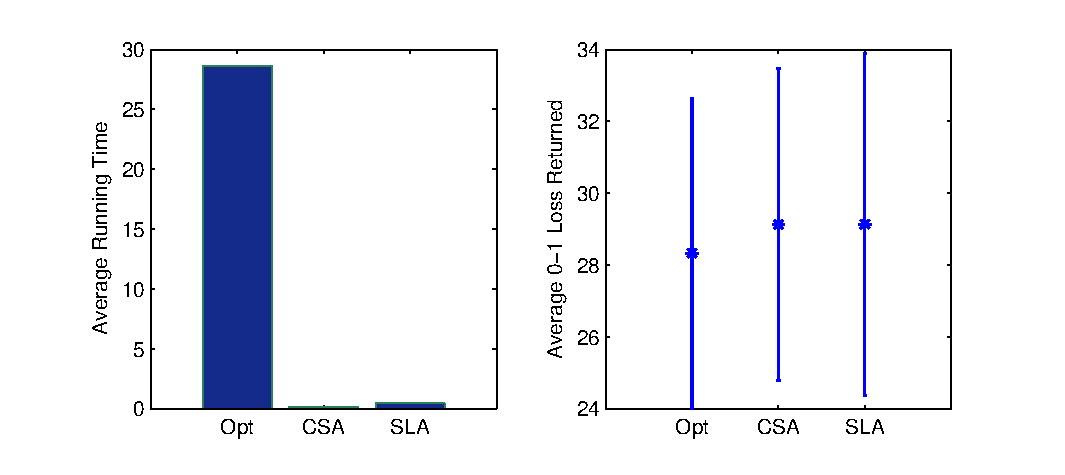
\includegraphics[width=0.50\textwidth]{images/fig54_approxsumm.eps}
\caption{
This plot compare the two approximation algorithm: combinatorial search approximation (CSA) with SLA. For reference, optimal solutions (Opt) returned by prioritized combinatorial search is also displayed. The results shown are based on average value of 30 synthetic datasets with $N=150$ and $D=3$. The left plot shows the average running times of CSA $(0.18 \pm 0.01)$, SLA $(0.45 \pm 0.26)$, and Opt $(28.66 \pm 0.24)$. The right plot shows the average loss values of returned solutions of CSA $(29.13 \pm 4.34)$, SLA $(29.13 \pm 4.75)$, and Opt $(28.33 \pm 4.32)$. It can be seen, that SLA and CSA have very similar accuracy in approximation, and both are quite close to the optimal solution. Figure \ref{fig:sla.approxlosses}, a continuation of this figure, also confirms this statement. 
}
\label{fig:sla.approxsumm}
\end{figure}

Sensible values for the constants given in Algorithm \ref{alg:sla.algorithm} are, for example, the followings:
\[ \begin{array} {lll}
& r_R = 2^{-1}, &R0 = 8, \\
& r_\epsilon = 2^{-1}, &\epsilon_{S0} = 0.2, \\
& r_K = 10, &K_{MIN} = 2, \quad K_{MAX} = 200.
\end{array} \] 
In this case the precision constant $K$ will gain values 2, 20, 200 in this given order. The corresponding values for radius $R$ are 8, 4, 2, and for the step size $\epsilon_S$ are 0.2, 0.1, 0.05. This setting seems to work well in practice for both data normalized to zero mean unit variance or squeezed into the $[0,1]$ range. This also works reasonably good for unnormalized data in many cases. In fact, this setting is used in all tests in this thesis where SLA algorithm is used, therefore it is verified by the good performance of SLA in those tests. For instance, Figure \ref{fig:sla.approxsumm} and Figure \ref{fig:sla.approxlosses} provides visual result of tests that compare the accuracy of the two approximation algorithms proposed in this thesis: the combinatorial search approximation (CSA) and SLA. The results shown in these figures are from 30 synthetic datasets of size $N=80$ and $D=3$. Also shown in these figures are optimal results given by running the prioritized combinatorial search as a reference. It can be seen from these figures, that CSA and SLA have very similar approximation accuracy, and both are quite close to the optimal solution. 



\begin{figure}[here]
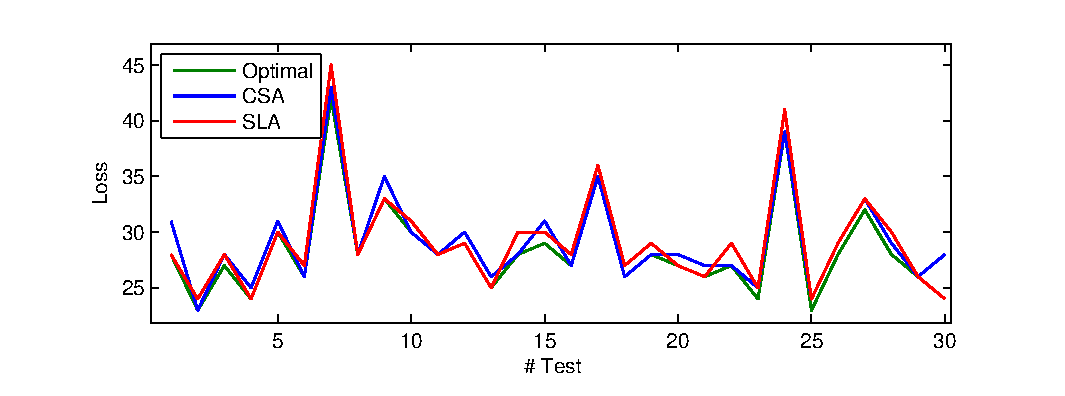
\includegraphics[width=0.50\textwidth]{images/fig55_approxlosses.eps}
\caption{
This figure is a continuation of Figure \ref{fig:sla.approxsumm} and shows the actual loss values of the solutions returned by the corresponding algorithm for each of the 30 synthetically generated datasets. The green curve corresponds to the optimal 0--1 loss value (determined by the prioritized combinatorial search algorithm). The blue curve corresponds to the loss value approximated by CSA, and the red curve by SLA. It can be seen that in some tests, SLA is better, while in other tests CSA is better, but the difference between these two are minimal, and on average they have about a same accuracy.
}
\label{fig:sla.approxlosses}
\end{figure}

\begin{figure}[here]
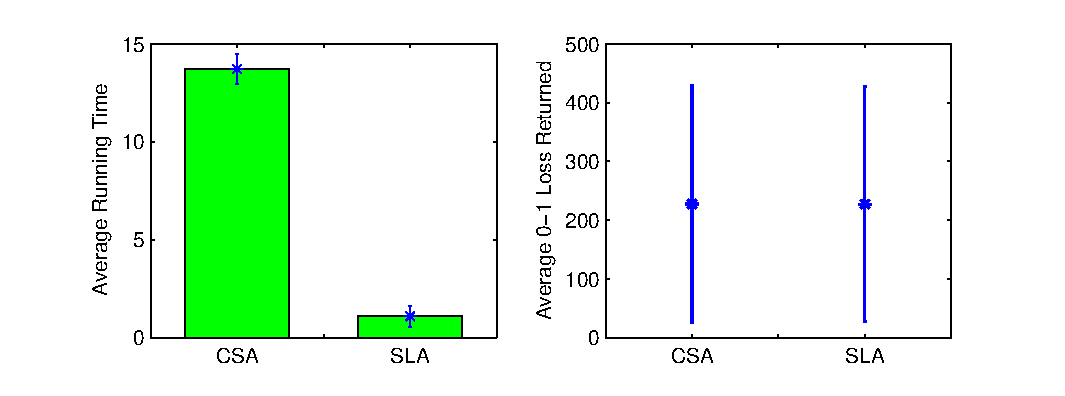
\includegraphics[width=0.50\textwidth]{images/fig56_approxsumm.eps}
\caption{
This figure compares the CSA and SLA algorithms using synthetic datasets of larger size. Results shown here are average value of tests on 30 datasets of size $N=5000$ and $D=8$. The right plot shows that SLA and CSA have similar approximation precision. The left plot, however, shows that the running time of SLA $(1.09 \pm 0.54)$ is much lower than that of CSA $(13.72 \pm 0.77)$.
}
\label{fig:sla.approxsumm2}
\end{figure}

As for the running time, CSA seems to outperform SLA in these tests as shown in the left plot of Figure \ref{fig:sla.approxsumm}. To decide this, a very similar test as the above was executed, except this time the synthetic datasets were much larger, with $N=5000$ and $D=8$. The constant $N'$ (to get initial best combination) of CSA was set to $2D$ (=16). The results is shown in Figure \ref{fig:sla.approxsumm2}. The right plot, again, shows that both algorithms have very similar accuracy. The plot on the left, however, shows that the running time of SLA $(1.09 \pm 0.54)$ is significantly lower than that of CSA $(13.72 \pm 0.77)$. Clearly, regarding running time, SLA is much more efficient than CSA. This will also be confirmed analytically in the next section.



%=================================================
\subsection{Performance Analysis of SLA Algorithm}
\label{sec:sla.performance}

The last test in the previous section showed (by Figure \ref{fig:sla.approxsumm2}), that for bigger datasets, the running time of SLA is considerably lower than that of CSA. This section will, therefore examine the complexity of the SLA algorithm analytically, and then compare it with that of CSA algorithm. 

Firstly, the complexity of function {\sc Gradient-Descent-in-Range} given by Algorithm \ref{alg:sla.range} is inspected, because it is the major component of the SLA algorithm. It is hard to derive the average complexity of this algorithm analytically, but the worst case complexity is easier to analyze as follows. The loop at step 2 and step 4 repeats for maximally $N/\epsilon_L$ times, because the loss value is upper bounded by $N$, and in each repeat of these loops, the loss is reduced by at least $\epsilon_L$. Inside the loop at step 4, the calculation of the smooth loss function and its gradient takes time $O(ND)$, the while loop at step 7 repeats exactly $O(log(max_{rate} / min_{rate}))$, which is a constant. In the second part of this function, the two for loops at step 15, 16 repeat exactly $(D+1) (2R/\epsilon_S)$ times. Inside these for loops, the calculation of smooth loss function takes time $O(ND)$. Thus, the second part (steps 15 to 23) takes times $O(ND^2)$, because $(2R/\epsilon_S)$ is just a constant. So, all together, the function {\sc Gradient-Descent-in-Range}  takes time $O(N^2D^2)$ in the worst case (when the loop at step 2 repeats for $N$ times).

Now, To identify the complexity of SLA algorithm, the code of Algorithm \ref{alg:sla.algorithm} is inspected as follows. In step 2, if linear SVM is used to give the initial approximation of $\w^*$, the complexity is $O(ND)$. Steps 3 -- 5 clearly take a constant time. The while loop at step 6 repeats for exactly $\log_{r_K} (K_{MAX} / K_{MIN})$ times. Inside this while loop, steps 8 -- 10 take a constant time, step 7 calls the function {\sc Gradient-Descent-in-Range}, which takes $O(N^2D^2)$ time. The whole algorithm is, therefore, $O(N^2D^2)$, because $\log_{r_K} (K_{MAX} / K_{MIN})$ -- the number of repeats of the while loop at step 6 -- is a constant. 

Clearly, comparing to the complexity $O(N^3D^2)$ of CSA algorithm, the complexity $O(N^2D^2)$ of SLA algorithm is much better. Note, that both these bounds are for the worst case scenario and the average performance should be much better, because in both cases, loops are broken immediately when a better solution is found. This statement is evidenced by Figure \ref{fig:sla.approxsumm2}, where it takes the SLA algorithm just slightly over a second, and CSA about 14 seconds, to solve problems of $N=5000$ and $D=8$, whereas a dummy loop that repeats just one operation $a = (2*3)/5.9$ for $N^2D^2 = 5000^28^2$ times takes 408.16 seconds to finish, and for $N^3D^2 = 5000^38^2$ it would clearly takes about $2.10^6$ seconds.


%=================================================
\subsection{Summary}
\label{sec:sla.summaryl}

In this chapter, the smooth loss function has been developed to approximate 0--1 loss function with controllable accuracy to (almost) any desired level of precision. Based on the characteristics of the smooth loss function, the SLA (smooth loss approximation) algorithm has been designed to approximate the optimal solution of 0--1 loss. It has been pointed out by different tests in this chapter, that SLA algorithm has comparable approximation accuracy as that of CSA (combinatorial search approximation), while SLA algorithm is much more efficient, especially for larger datasets. This is confirmed by the provided performance analysis, which shows that the worst cases complexity of SLA is $O(N^2D^2)$, whereas for CSA it is$O(N^3D^2)$. Practical tests, however, showed that the average running time of both algorithms is significantly lower than the given worst case scenario. Many more tests and comparison will be conducted in the next chapter. 

